\begin{center}
\Huge
Konfidensinterval og binomialtest
\end{center}
\section*{Konfidensintervaller}
\stepcounter{section}
%Overskrift
\begin{setn}
Har vi en binomialfordelt stikprøve på $n$ elementer med sandsynlighedsparameter $p$, så er et $95\%$ konfidensinterval givet ved
\begin{align*}
\left[ \hat{p} - 2\sqrt{\frac{\hat{p}(1-\hat{p})}{n}};\hat{p} + 2\sqrt{\frac{\hat{p}(1-\hat{p})}{n}}\right],
\end{align*}
hvor $\hat{p}$ er stikprøveestimatet for $p$. 
\end{setn}
Dette skal forstås på følgende måde. Laver vi en stikprøve på $n$ elementer 100 gange, så vil vi få 100 forskellige konfidensintervaller. Så vil vi forvente at den rigtige $p$ vil ligge inde i $95$ af disse $100$ konfidensintervaller.

\section*{Hypotesetest}
\stepcounter{section}
Vi har for nogle år siden spurgt 900 personer om deres holdning til et byggeprojekt i lokalområdet. 48$\%$ var imod projektet. Vi forventer derfor, at antallet af utilfredse personer følger en binomialfordeling med antalsparameter $900$ og $p = 0,48$. Vi spørger nu igen befolkningen, og denne gang er $52\%$ utilfredse. Vi opstiller derfor en nul-hypotese $H_0:$ Holdningen til byggeprojektet har ikke ændret sig. Den alternative hypotese $H_1$ er så: Modstanden mod byggeprojektet er steget. 

Vi ønsker at bestemme sandsynligheden for $H_0$ og hvis den er mindre end et \textit{signifikansniveau} på $5\%$, så vil vi forkaste nulhypotesen. 
Vi bestemmer derfor sandsynligheden for, at mere end $900\cdot 0.52 = 468$ personer er utilfredse, hvis de følger en binomialfordeling med $n=900$ og $p = 0.48$. Dette gøres i Maple med \texttt{bincdf(900,0.48,468,$\infty$)} og giver 
$0,00895$ eller 0,895$\%$. Derfor forkaster vi nulhypotesen at holdningen ikke har ændret sig. 

Vi kan bestemme alle de udfald af antal personer der udtrykker modstand, der vil gøre, at vi vil forkaste nulhypotesen ved \texttt{binomialTest(900,0.48,0.05,højre)}. Dette giver os plottet på Fig. \ref{fig:højretest}.
\begin{figure}[H]
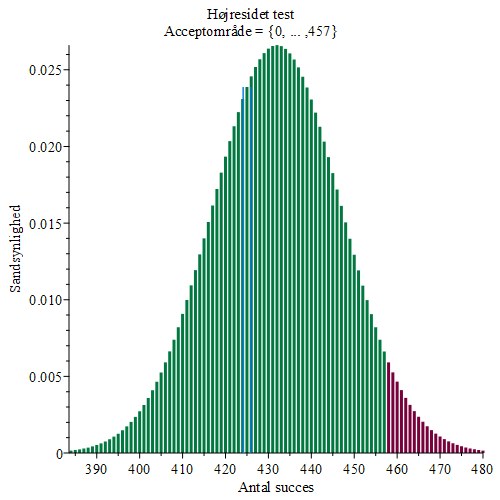
\includegraphics[width=\textwidth]{Billeder/binomialtest.png}
\caption{Højresidet test på stemmefordeling}
\label{fig:højretest}
\end{figure}

Vi kan derfor se, at alle udfald $X\geq 457$ vil gøre, at vi tror på nulhypotesen. Tilsvarende vil alle udfald $X\geq 458$ vil gøre, at vi forkaster nulhypotesen. Mængden $\{458,\hdots,900\}$ kaldes for den kritiske mængde. 

\section*{Opgave 1}
\begin{enumerate}[label=\roman*)]
\item En producent af et lægemiddel påstår, at $12\%$ af anvendelserne af lægemiddelet er succesfulde. Ud af 100 personer bliver kun 5 helbredt. Vores nulhypotese er, at producenten taler sandt. Med et signifikansniveau på $5\%$, vil vi så forkaste nulhypotesen? Hvad er den kritiske mængde for forsøget?
\item Til seneste valg spurgte vi 300 personer om, hvad de stemte. 30 stemte på liste Q. Vi har nu spurgt 300 nye personer og denne gang har partiet fået 25 stemmer. Er det rimeligt at antage, at partiets vælgertilslutning er faldet? Hvis vores nulhypotese er, at tilslutningen ikke er faldet, kan vi så med et signifikansniveau på $5\%$ forkaste denne nulhypotese? Bestem desuden den kritiske mængde
\item En mand finder 3 sten i sit glas med oliven og synes, at det er lidt for mange. Han kigger på glasset, og der er det lovet, at glasset er $99\%$ stenfri. I glasset er der 70 oliven. Har han grund til sin skepsis? Opstil nulhypotese og se, om den kan forkastes med et signifikansniveau på $5\%$. Bestem desuden den kritiske mængde. 
\item Vi kaster med en mønt, og vil se, om plat og krone er lige sandsynlige. Vi slår 150 gange og får plat 72 gange. Nulhypotesen er $H_0$: Plat og krone er lige sandsynlige. Bestem med et signifikansniveau på $5\%$ om vi vil forkaste nulhypotesen. Bestem desuden den kritiske mængde. 
\end{enumerate}

\section*{Opgave 2}
En butik har et klientel, der består af $30\%$ mænd. 
\begin{enumerate}[label=\roman*)]
\item Opstil en binomialmodel, der beskriver antallet af mænd i en stikprøve på $50$ personer.
\item Hvad er sandsynligheden for, at 12 af personerne i stikprøven er mænd?
\item En dag havde butikken $220$ kunder. 79 af disse var mænd. Opstil en nulhypotese, der beskriver undersøgelsen, og brug en binomialtest med et signifikansniveau på $5\%$ til at undersøge nulhypotesen. 
\end{enumerate}

\section*{Opgave 3}
Spørg mig